\subsection{Escenario Experimental A} \label{sec:EscenarioExperimentalA}

El primer escenario, busca el evaluar la capacidad de la implementación realizada de iniciar toda una aplicación desde cero. Partiendo de esto, se definió la aplicación vista en la figura \ref{fig:ExpA}. Esta tiene dos locaciones raíz, con requerimientos de datos iguales en ambas.

\begin{figure}[H]
    \centering
    \caption{\\Diagrama del escenario experimental A}
    \label{fig:ExpA}
    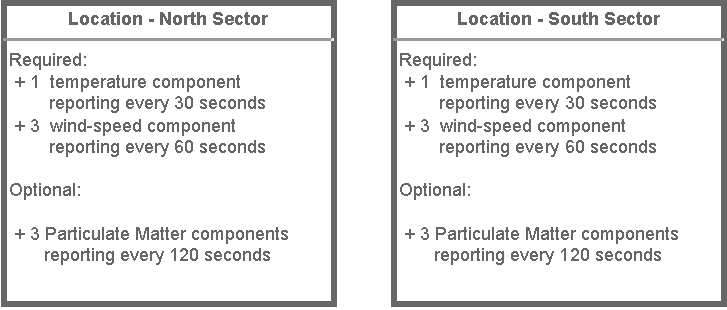
\includegraphics[width=0.8\linewidth]{images/ScenarioA.pdf}
    \vspace{-4mm}
\end{figure}

Inicialmente, no habrán dispositivos presentes en ejecución, por lo que el sistema tendrá que identificar la falla, definir las acciones de adición correspondientes, y ejecutarlas para poder suplir con los requerimientos de datos.

Para ello, tomando como referencia la figura \ref{fig:ExpA}, se realizó la declaración del estado de referencia, presente en el anexo \ref{ape:ExpA}, y, como observa en la figura \ref{fig:ValidA}, se validó usando \textit{Lexical}.

\begin{figure}[H]
    \centering
    \caption{\\Validación de la declaración de referencia realizada para el escenario experimental A}
    \label{fig:ValidA}
    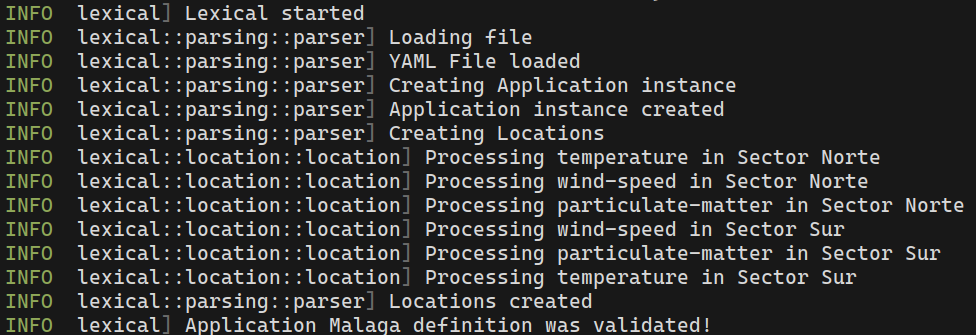
\includegraphics[width=0.7\linewidth]{images/ValidationLexicalA.png}
    \vspace{-4mm}
\end{figure}

Ya con las condiciones iniciales, y el estado de referencia definido, se estructuraron, las directivas, vistas en el anexo \ref{ape:DirectivesA}, que permitirían realizar la adaptación de la arquitectura hacia el estado de objetivo. 

Partiendo de todo lo anterior, se definió la serie de pasos a realizar para este primer escenario experimental:

\begin{enumerate}[itemsep=0mm]
    \item Desplegar los servicios de Smart Campus UIS
    \item Desplegar los servicios \textit{Bran} y \textit{DoThing}.
    \item Usando \textit{Lexical}, establecer el estado de referencia de la aplicación.
    \item Declarar en los endpoints de \textit{Bran}, las directivas definidas.
    \item Desplegar el servicio \textit{Looker} para la aplicación.
    \item A la nivelación del estado de la aplicación.
\end{enumerate}

Al final de la simulación de este escenario, se eliminarán todos los servicios desplegados con el fin de asegurar una ejecución limpia de futuros procesos.
